\section{Referentni podaci}

Referentni podaci su oni podaci s kojima se uspoređuju rezultati metoda. Ti referentni podaci su generirani u simulatoru te predstavljaju lokaciju i rotaciju vozila u jednome trenutku. Referentni podaci se zapravo sastoje od lokacije i rotacije vozila.

\subsubsection{Lokacija}
Lokacija vozila je također definirana kao točka u kartezijevom koordinatnome prostoru. Sastoji se od x, y i z koordinata. Slično kao prikazano na slici \ref{fig:point_coordinates}.


\subsubsection{Rotacija}
 U trodimenzialnome prostoru objekt se zapravo može rotirati oko beskonaćnoga broja osi ali se u pravilu uzimaju 3 statičke osi. Te osi se nazivaju os skretanja (eng. yaw), os poniranja (eng. pitch) i os valjanja (eng. roll). 

\begin{figure}[!ht]
  \centering
  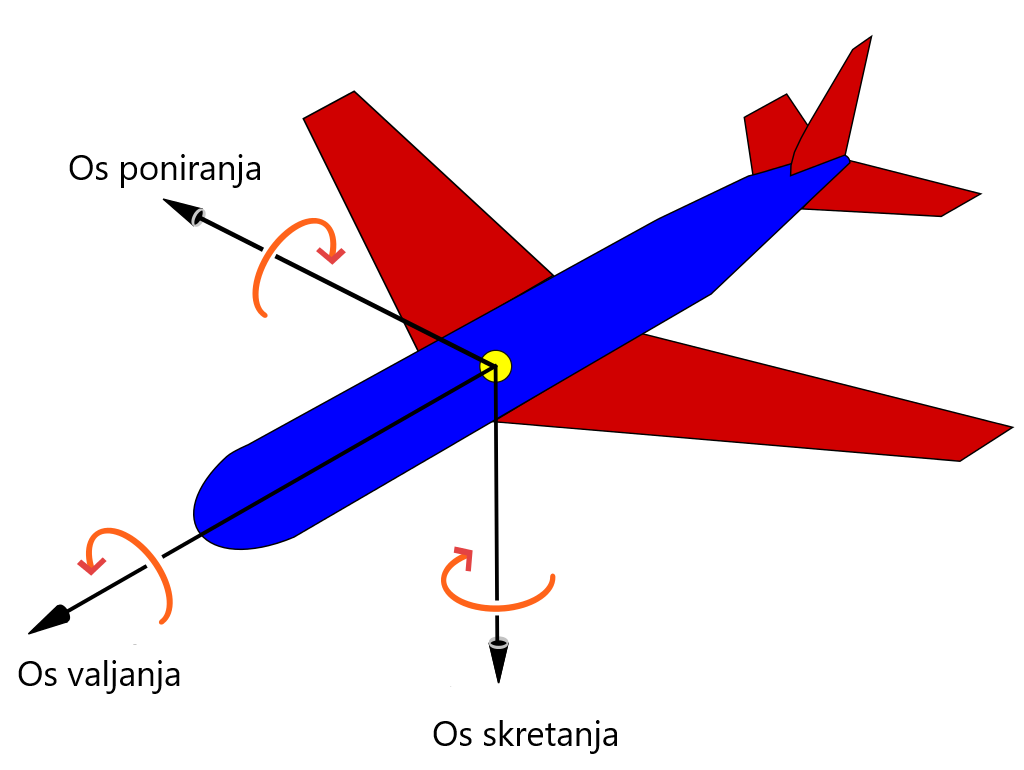
\includegraphics[scale=0.3]{images/yaw_roll_pitch_example.png}
  \caption{Ilustracija osi rotiranja}
  \label{fig:yaw_roll_pitch_example}
\end{figure}


Os rotacije je os koja prolazi u smjeru kretanja vozila (x os), os poniranja je zapravo os okomita s os rotacija (z os), dok je os skretanja okomita na obje prethodne osi (y os). Te osi su ilustrirane na slici \ref{fig:yaw_roll_pitch_example}.

Vizualizacije referentnih podataka za jedan primjer kretanja vozila možemo vidjeti na sljedećim slikama. Na svim grafovima svaka točka predstavlja jedno očitanje. Grafovi su izgrađeni pomoću programskog jezika Kotlin koristeći biblioteku XChart. Slika \ref{fig:gt_lokacija} prikazuje graf lokacija vozila. Slika \ref{fig:gt_lokacija_x} pokazuje x koordinate vozila  uvremenu. Slika \ref{fig:gt_lokacija_y} pokazuje y koordinate vozila u vremenu. Slika \ref{fig:gt_rotacija} pokazuje vrijednosti rotacija oko statičkih osi u vremenu. Za očekivati je kako će se mjenjati samo rotacija skretanja zato što vozilo može skretati, a ne može ponirati ili se valjati. 

\begin{figure}[h!]
  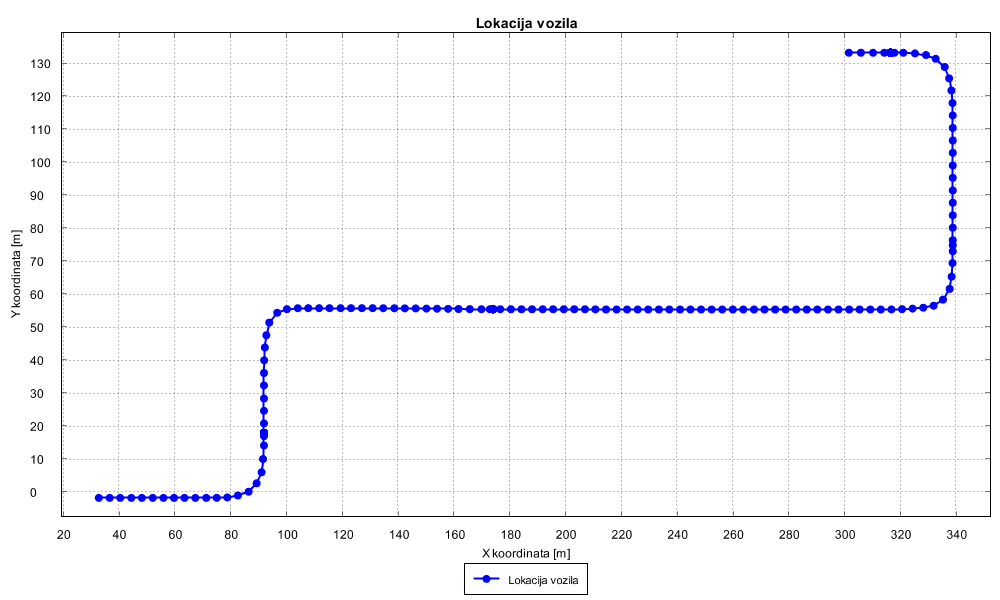
\includegraphics[scale=0.4]{images/gt_lokacija.png}
  \caption{Graf lokacije vozila}
  \label{fig:gt_lokacija}
\end{figure}
\pagebreak
\begin{figure}[h!]
  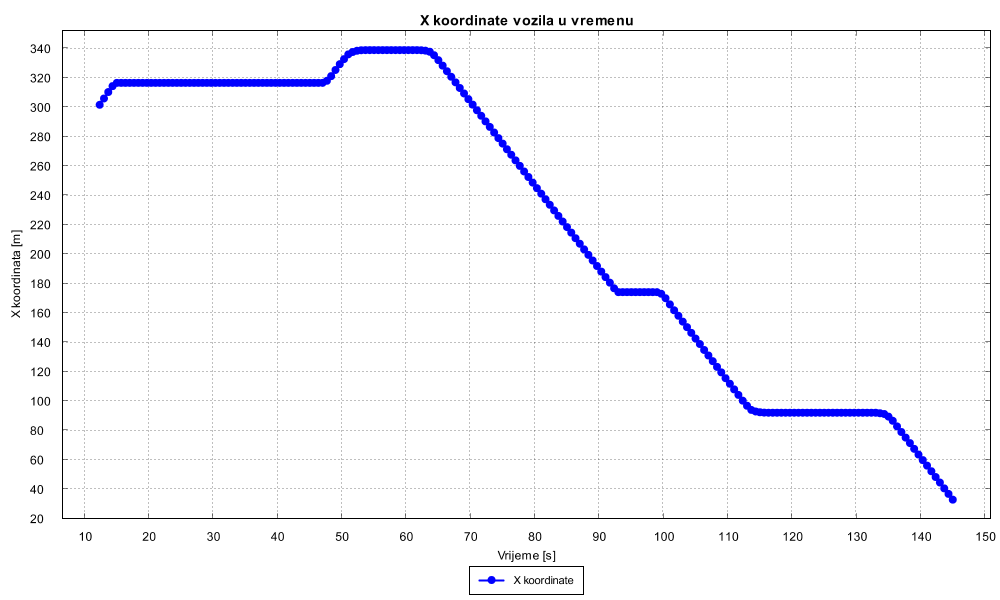
\includegraphics[scale=0.4]{images/gt_lokacija_x.png}
  \caption{Graf X lokacije vozila u vremenu}
  \label{fig:gt_lokacija_x}
\end{figure}
\begin{figure}[h!]
  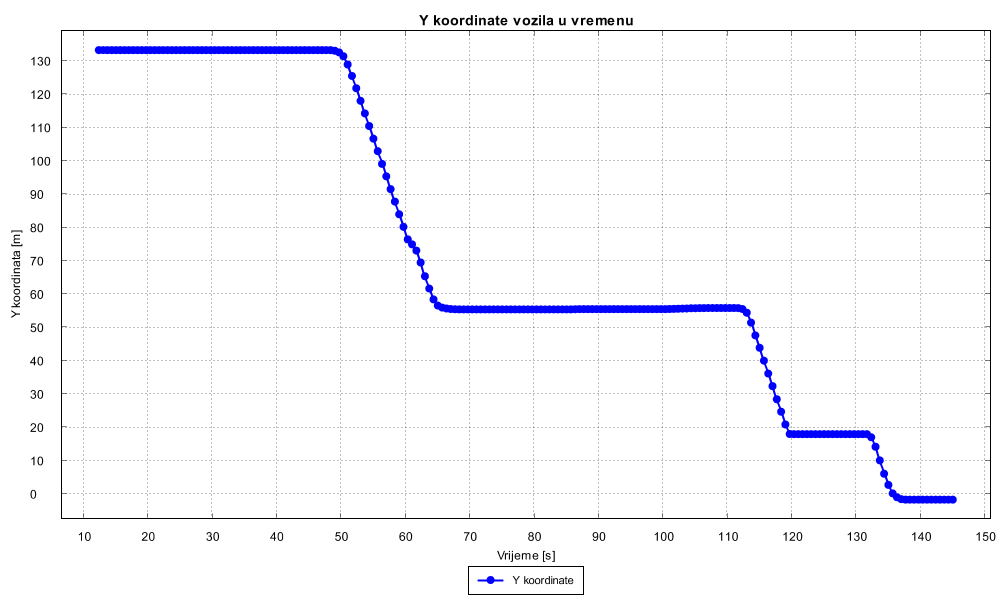
\includegraphics[scale=0.4]{images/gt_lokacija_y.png}
  \caption{Graf Y lokacije vozila u vremenu}
  \label{fig:gt_lokacija_y}
\end{figure}
\pagebreak
\begin{figure}[h!]
  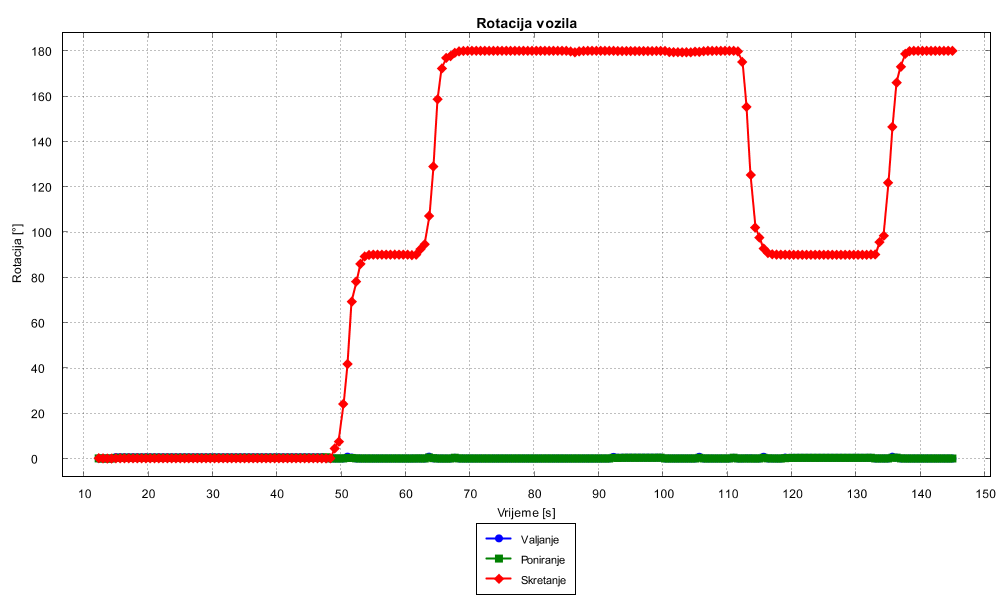
\includegraphics[scale=0.4]{images/gt_rotacija.png}
  \caption{Graf rotacija u vremenu}
  \label{fig:gt_rotacija}
\end{figure}